% Name: Tax and deadweight loss
% Description: A per-unit tax on sellers shifts supply up by the tax: buyers pay more, sellers keep less, the government collects the rectangle, and the triangle of trades that no longer happen is the deadweight loss.
% Tags: tax incidence, deadweight loss, tax revenue, welfare, microeconomics

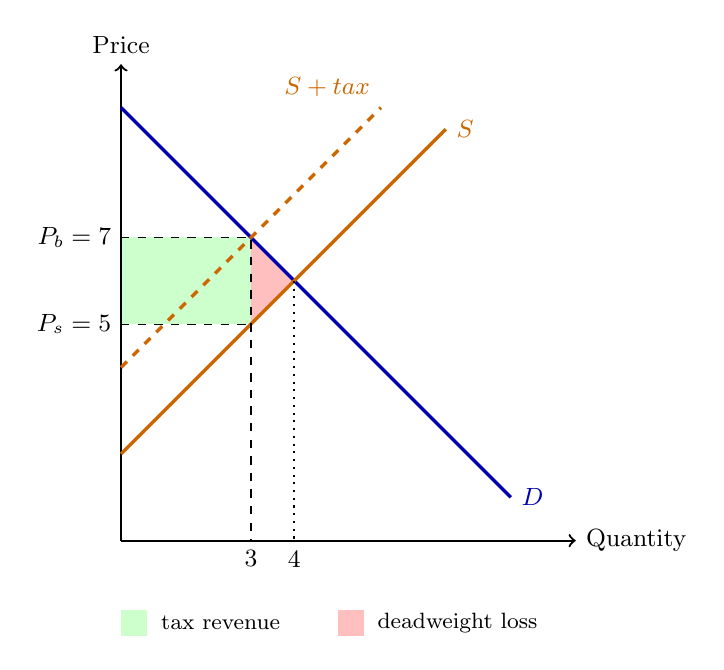
\begin{tikzpicture}[scale=0.55, every node/.style={font=\small}]
  % D: P = 10 - Q, S: P = 2 + Q, and with a tax of 2, S + tax: P = 4 + Q, which meets D at Q = 3, where buyers pay 7 and sellers keep 5
  \fill[green!20] (0,5) rectangle (3,7);
  \fill[red!25] (3,7) -- (3,5) -- (4,6) -- cycle;
  \draw[->, thick] (0,0) -- (10.5,0) node[right] {Quantity};
  \draw[->, thick] (0,0) -- (0,11) node[above] {Price};
  \draw[very thick, blue!70!black] (0,10) -- (9,1) node[right] {$D$};
  \draw[very thick, orange!80!black] (0,2) -- (7.5,9.5) node[right] {$S$};
  \draw[very thick, orange!80!black, dashed] (0,4) -- (6,10) node[above left] {$S + \text{tax}$};
  \draw[dashed] (0,7) node[left] {$P_b = 7$} -| (3,0) node[below] {$3$};
  \draw[dashed] (0,5) node[left] {$P_s = 5$} -- (3,5);
  \draw[dotted, thick] (4,6) -- (4,0) node[below] {$4$};
  % Swatches under the axis name the shaded areas
  \fill[green!20] (0,-2.2) rectangle ++(0.6,0.6);
  \node[anchor=west, font=\footnotesize] at (0.7,-1.9) {tax revenue};
  \fill[red!25] (5,-2.2) rectangle ++(0.6,0.6);
  \node[anchor=west, font=\footnotesize] at (5.7,-1.9) {deadweight loss};
\end{tikzpicture}
